%  LaTeX support: latex@mdpi.com 
%  For support, please attach all files needed for compiling as well as the log file, and specify your operating system, LaTeX version, and LaTeX editor.

%=================================================================
\documentclass[journal,article,submit,pdftex,moreauthors]{Definitions/mdpi} 

%--------------------
% Class Options:
%--------------------
%----------
% journal
%----------
% Choose between the following MDPI journals:
% acoustics, actuators, addictions, admsci, adolescents, aerobiology, aerospace, agriculture, agriengineering, agrochemicals, agronomy, ai, air, algorithms, allergies, alloys, analytica, analytics, anatomia, animals, antibiotics, antibodies, antioxidants, applbiosci, appliedchem, appliedmath, applmech, applmicrobiol, applnano, applsci, aquacj, architecture, arm, arthropoda, arts, asc, asi, astronomy, atmosphere, atoms, audiolres, automation, axioms, bacteria, batteries, bdcc, behavsci, beverages, biochem, bioengineering, biologics, biology, biomass, biomechanics, biomed, biomedicines, biomedinformatics, biomimetics, biomolecules, biophysica, biosensors, biotech, birds, bloods, blsf, brainsci, breath, buildings, businesses, cancers, carbon, cardiogenetics, catalysts, cells, ceramics, challenges, chemengineering, chemistry, chemosensors, chemproc, children, chips, cimb, civileng, cleantechnol, climate, clinpract, clockssleep, cmd, coasts, coatings, colloids, colorants, commodities, compounds, computation, computers, condensedmatter, conservation, constrmater, cosmetics, covid, crops, cryptography, crystals, csmf, ctn, curroncol, cyber, dairy, data, ddc, dentistry, dermato, dermatopathology, designs, devices, diabetology, diagnostics, dietetics, digital, disabilities, diseases, diversity, dna, drones, dynamics, earth, ebj, ecologies, econometrics, economies, education, ejihpe, electricity, electrochem, electronicmat, electronics, encyclopedia, endocrines, energies, eng, engproc, entomology, entropy, environments, environsciproc, epidemiologia, epigenomes, est, fermentation, fibers, fintech, fire, fishes, fluids, foods, forecasting, forensicsci, forests, foundations, fractalfract, fuels, future, futureinternet, futurepharmacol, futurephys, futuretransp, galaxies, games, gases, gastroent, gastrointestdisord, gels, genealogy, genes, geographies, geohazards, geomatics, geosciences, geotechnics, geriatrics, grasses, gucdd, hazardousmatters, healthcare, hearts, hemato, hematolrep, heritage, higheredu, highthroughput, histories, horticulturae, hospitals, humanities, humans, hydrobiology, hydrogen, hydrology, hygiene, idr, ijerph, ijfs, ijgi, ijms, ijns, ijpb, ijtm, ijtpp, ime, immuno, informatics, information, infrastructures, inorganics, insects, instruments, inventions, iot, j, jal, jcdd, jcm, jcp, jcs, jcto, jdb, jeta, jfb, jfmk, jimaging, jintelligence, jlpea, jmmp, jmp, jmse, jne, jnt, jof, joitmc, jor, journalmedia, jox, jpm, jrfm, jsan, jtaer, jvd, jzbg, kidneydial, kinasesphosphatases, knowledge, land, languages, laws, life, liquids, literature, livers, logics, logistics, lubricants, lymphatics, machines, macromol, magnetism, magnetochemistry, make, marinedrugs, materials, materproc, mathematics, mca, measurements, medicina, medicines, medsci, membranes, merits, metabolites, metals, meteorology, methane, metrology, micro, microarrays, microbiolres, micromachines, microorganisms, microplastics, minerals, mining, modelling, molbank, molecules, mps, msf, mti, muscles, nanoenergyadv, nanomanufacturing,\gdef\@continuouspages{yes}} nanomaterials, ncrna, ndt, network, neuroglia, neurolint, neurosci, nitrogen, notspecified, %%nri, nursrep, nutraceuticals, nutrients, obesities, oceans, ohbm, onco, %oncopathology, optics, oral, organics, organoids, osteology, oxygen, parasites, parasitologia, particles, pathogens, pathophysiology, pediatrrep, pharmaceuticals, pharmaceutics, pharmacoepidemiology,\gdef\@ISSN{2813-0618}\gdef\@continuous pharmacy, philosophies, photochem, photonics, phycology, physchem, physics, physiologia, plants, plasma, platforms, pollutants, polymers, polysaccharides, poultry, powders, preprints, proceedings, processes, prosthesis, proteomes, psf, psych, psychiatryint, psychoactives, publications, quantumrep, quaternary, qubs, radiation, reactions, receptors, recycling, regeneration, religions, remotesensing, reports, reprodmed, resources, rheumato, risks, robotics, ruminants, safety, sci, scipharm, sclerosis, seeds, sensors, separations, sexes, signals, sinusitis, skins, smartcities, sna, societies, socsci, software, soilsystems, solar, solids, spectroscj, sports, standards, stats, std, stresses, surfaces, surgeries, suschem, sustainability, symmetry, synbio, systems, targets, taxonomy, technologies, telecom, test, textiles, thalassrep, thermo, tomography, tourismhosp, toxics, toxins, transplantology, transportation, traumacare, traumas, tropicalmed, universe, urbansci, uro, vaccines, vehicles, venereology, vetsci, vibration, virtualworlds, viruses, vision, waste, water, wem, wevj, wind, women, world, youth, zoonoticdis 
% For posting an early version of this manuscript as a preprint, you may use "preprints" as the journal. Changing "submit" to "accept" before posting will remove line numbers.

%---------
% article
%---------
% The default type of manuscript is "article", but can be replaced by: 
% abstract, addendum, article, book, bookreview, briefreport, casereport, comment, commentary, communication, conferenceproceedings, correction, conferencereport, entry, expressionofconcern, extendedabstract, datadescriptor, editorial, essay, erratum, hypothesis, interestingimage, obituary, opinion, projectreport, reply, retraction, review, perspective, protocol, shortnote, studyprotocol, systematicreview, supfile, technicalnote, viewpoint, guidelines, registeredreport, tutorial
% supfile = supplementary materials

%----------
% submit
%----------
% The class option "submit" will be changed to "accept" by the Editorial Office when the paper is accepted. This will only make changes to the frontpage (e.g., the logo of the journal will get visible), the headings, and the copyright information. Also, line numbering will be removed. Journal info and pagination for accepted papers will also be assigned by the Editorial Office.

%------------------
% moreauthors
%------------------
% If there is only one author the class option oneauthor should be used. Otherwise use the class option moreauthors.

%---------
% pdftex
%---------
% The option pdftex is for use with pdfLaTeX. Remove "pdftex" for (1) compiling with LaTeX & dvi2pdf (if eps figures are used) or for (2) compiling with XeLaTeX.

%=================================================================
% MDPI internal commands - do not modify
\firstpage{1} 
\makeatletter 
\setcounter{page}{\@firstpage} 
\makeatother
\pubvolume{1}
\issuenum{1}
\articlenumber{0}
\pubyear{2024}
\copyrightyear{2023}
%\externaleditor{Academic Editor: Firstname Lastname}
\datereceived{ } 
\daterevised{ } % Comment out if no revised date
\dateaccepted{ } 
\datepublished{ } 
%\datecorrected{} % For corrected papers: "Corrected: XXX" date in the original paper.
%\dateretracted{} % For corrected papers: "Retracted: XXX" date in the original paper.
\hreflink{https://doi.org/} % If needed use \linebreak
%\doinum{}
%\pdfoutput=1 % Uncommented for upload to arXiv.org
%\CorrStatement{yes}  % For updates


%=================================================================
% Add packages and commands here. The following packages are loaded in our class file: fontenc, inputenc, calc, indentfirst, fancyhdr, graphicx, epstopdf, lastpage, ifthen, float, amsmath, amssymb, lineno, setspace, enumitem, mathpazo, booktabs, titlesec, etoolbox, tabto, xcolor, colortbl, soul, multirow, microtype, tikz, totcount, changepage, attrib, upgreek, array, tabularx, pbox, ragged2e, tocloft, marginnote, marginfix, enotez, amsthm, natbib, hyperref, cleveref, scrextend, url, geometry, newfloat, caption, draftwatermark, seqsplit
% cleveref: load \crefname definitions after \begin{document}

%=================================================================
% Please use the following mathematics environments: Theorem, Lemma, Corollary, Proposition, Characterization, Property, Problem, Example, ExamplesandDefinitions, Hypothesis, Remark, Definition, Notation, Assumption
%% For proofs, please use the proof environment (the amsthm package is loaded by the MDPI class).

%=================================================================
% Full title of the paper (Capitalized)
\Title{The Dynamics of Polluted Black Holes: Implications for Accretion Processes and Tidal Disruption Events}

% MDPI internal command: Title for citation in the left column
\TitleCitation{The Dynamics of Polluted Black Holes: Implications for Accretion Processes and Tidal Disruption Events}

% Author Orchid ID: enter ID or remove command
\newcommand{\orcidauthorA}{0000-0002-1109-9662} % Add \orcidA{} behind the author's name
%\newcommand{\orcidauthorB}{0000-0000-0000-000X} % Add \orcidB{} behind the author's name

% Authors, for the paper (add full first names)
\Author{Raghav Chari $^{1,}$*\orcidA{} and Apurva Oza $^{2}$}

%\longauthorlist{yes}

% MDPI internal command: Authors, for metadata in PDF
\AuthorNames{Raghav Chari and Apurva Oza}

% MDPI internal command: Authors, for citation in the left column
\AuthorCitation{Chari, R.; Oza, A.}
% If this is a Chicago style journal: Lastname, Firstname, Firstname Lastname, and Firstname Lastname.

% Affiliations / Addresses (Add [1] after \address if there is only one affiliation.)
\address{%
$^{1}$ \quad Department of Physics and Astronomy, University of Tennessee, Knoxville, TN 37996-1200;\\
$^{2}$ \quad Jet Propulsion Laboratory, California Institute of Technology, Pasadena, CA 91109, USA;}

% Contact information of the corresponding author
\corres{Correspondence: rchari1@tennessee.edu}

% Current address and/or shared authorship
% The commands \thirdnote{} till \eighthnote{} are available for further notes

%\simplesumm{} % Simple summary

%\conference{} % An extended version of a conference paper

% Abstract (Do not insert blank lines, i.e. \\) 
\abstract{Mass accretion is generally modeled as a two-body system with a satellite M$_2$ accreting $\dot{M}$ onto a primary M$_1$, the central object . Studying the physical mechanisms generically across a range of masses, provides insight into the energetics of such systems in the Universe. We consider high-mass objects orbiting a primary (e.g. star- black hole) as well as low-mass objects orbiting primaries (e.g. exomoon-exoplanet) focusing on the metallicity $\chi$ which can in principle, be observed. Test cases include the presence of metals in gas giants, as well as the accretion disks around black holes. Our research explores the concept of tidal disruption events (TDEs) and the associated accretion disk formation for all objects.
The study combines numerical simulations and analytic models, with the aim of making robust predictions on the particles in gas giant atmospheres,  products' which may be detectable spectrally today. Our results may inform future observations and detection strategies, and deepen our understanding of TDEs, exomoon composition, and the complex dynamics of accretion processes. At the larger scale, we find that the magnetospheric physics governing exoplanet-exomoon interactions may be informed by black holes as well.}

% Keywords
\keyword{Black Holes; Tidal Disruption Events; Accretion, Metalicity} 

% The fields PACS, MSC, and JEL may be left empty or commented out if not applicable
%\PACS{J0101}
%\MSC{}
%\JEL{}

%%%%%%%%%%%%%%%%%%%%%%%%%%%%%%%%%%%%%%%%%%
% Only for the journal Diversity
%\LSID{\url{http://}}

%%%%%%%%%%%%%%%%%%%%%%%%%%%%%%%%%%%%%%%%%%
% Only for the journal Applied Sciences
%\featuredapplication{Authors are encouraged to provide a concise description of the specific application or a potential application of the work. This section is not mandatory.}
%%%%%%%%%%%%%%%%%%%%%%%%%%%%%%%%%%%%%%%%%%

%%%%%%%%%%%%%%%%%%%%%%%%%%%%%%%%%%%%%%%%%%
% Only for the journal Data
%\dataset{DOI number or link to the deposited data set if the data set is published separately. If the data set shall be published as a supplement to this paper, this field will be filled by the journal editors. In this case, please submit the data set as a supplement.}
%\datasetlicense{License under which the data set is made available (CC0, CC-BY, CC-BY-SA, CC-BY-NC, etc.)}

%%%%%%%%%%%%%%%%%%%%%%%%%%%%%%%%%%%%%%%%%%
% Only for the journal Toxins
%\keycontribution{The breakthroughs or highlights of the manuscript. Authors can write one or two sentences to describe the most important part of the paper.}

%%%%%%%%%%%%%%%%%%%%%%%%%%%%%%%%%%%%%%%%%%
% Only for the journal Encyclopedia
%\encyclopediadef{For entry manuscripts only: please provide a brief overview of the entry title instead of an abstract.}

%%%%%%%%%%%%%%%%%%%%%%%%%%%%%%%%%%%%%%%%%%
% Only for the journal Advances in Respiratory Medicine
%\addhighlights{yes}
%\renewcommand{\addhighlights}{%

%\noindent This is an obligatory section in “Advances in Respiratory Medicine”, whose goal is to increase the discoverability and readability of the article via search engines and other scholars. Highlights should not be a copy of the abstract, but a simple text allowing the reader to quickly and simplified find out what the article is about and what can be cited from it. Each of these parts should be devoted up to 2~bullet points.\vspace{3pt}\\
%\textbf{What are the main findings?}
% \begin{itemize}[labelsep=2.5mm,topsep=-3pt]
% \item First bullet.
% \item Second bullet.
% \end{itemize}\vspace{3pt}
%\textbf{What is the implication of the main finding?}
% \begin{itemize}[labelsep=2.5mm,topsep=-3pt]
% \item First bullet.
% \item Second bullet.
% \end{itemize}
%}

%%%%%%%%%%%%%%%%%%%%%%%%%%%%%%%%%%%%%%%%%%
\begin{document}

%%%%%%%%%%%%%%%%%%%%%%%%%%%%%%%%%%%%%%%%%%


\section{Introduction}
\subsection{Stellar Pollution}

The phenomenon of pollution in stellar bodies, especially in white dwarfs, has garnered significant scientific interest in recent years. Studies like those conducted by Doyle et al. (2021) \cite{Doyle_2021} have played a pivotal role in deepening our understanding of this process. Stellar pollution typically involves the absorption of celestial bodies, such as planets and moons, into stars. This absorption significantly impacts the stellar composition and can provide valuable insights into the history and evolution of these celestial systems.

An intriguing aspect of this phenomenon is observed in the case of exo-Ios. These are moons with toroidal atmospheres, often around exoplanets. Oza et al. (2019) \cite{Oza_2019} demonstrates that these exo-Ios, which exhibit volcanic activity, contribute to the pollution of their stellar environments. This finding underscores the complexity of interactions within stellar systems and the varied sources of stellar pollution.

While much of the research on stellar pollution has focused on stars, black holes present a markedly different scenario. Their strong gravitational pulls and the presence of event horizons introduce unique dynamics compared to typical stars. This distinction leads to intriguing questions regarding the fate of celestial bodies, particularly exomoons, when they are captured by black holes.
\subsection{Polluted Black Holes}

The study of accretion disks around black holes is essential to understanding the complex physics of matter accumulation in these massive celestial bodies (e.g., Pringle et al. \cite{Pringle_1981}, Blandford and Payne \cite{Blandford_Payne_1982}, Artimage\cite{Armitage_2004}). Foundational work in this area, (eg., Armitage \cite{Armitage_2004}, Rees, \cite{Rees_1988}) and others, illuminates the interplay of gravitational, centrifugal, and viscous forces within these disks. This interplay results in differential rotation and the inward spiraling of matter toward the central black hole.



Near black holes, the dynamics of accretion disks are further complicated by the intense gravitational fields and the consequential relativistic effects. These factors make the study of matter accumulation near black holes, particularly the accretion of exomoons, a complex and fascinating subject.

Understanding the dynamics of accretion disks around black holes is crucial for analyzing how exomoons are captured and potentially accreted by these massive celestial bodies. This study aims to explore the potential evidence of icy exomoons falling into black hole accretion disks and their consequent pollution. By examining this process, we can gain insights into the dynamic environment surrounding black holes and possibly identify observational signatures indicative of exomoons in these extreme environments. This novel approach extends the concept of spallogenic nuclides, previously associated with the accretion of icy exomoons in white dwarfs, to the context of black holes.

%%%%%%%%%%%%%%%%%%%%%%%%%%%%%%%%%%%%%%%%%%
\section{Materials and Methods}
\subsection{SERPENS}

Meyer zu Westram et al. 2023 (submitted) \cite{Meyer_zu_Westram} studies the random velocity distribution of particles in free space. SERPENS employs a test particle algorithm on a 4-D grid (r, $\phi$, z, t).

\begin{figure}[H]
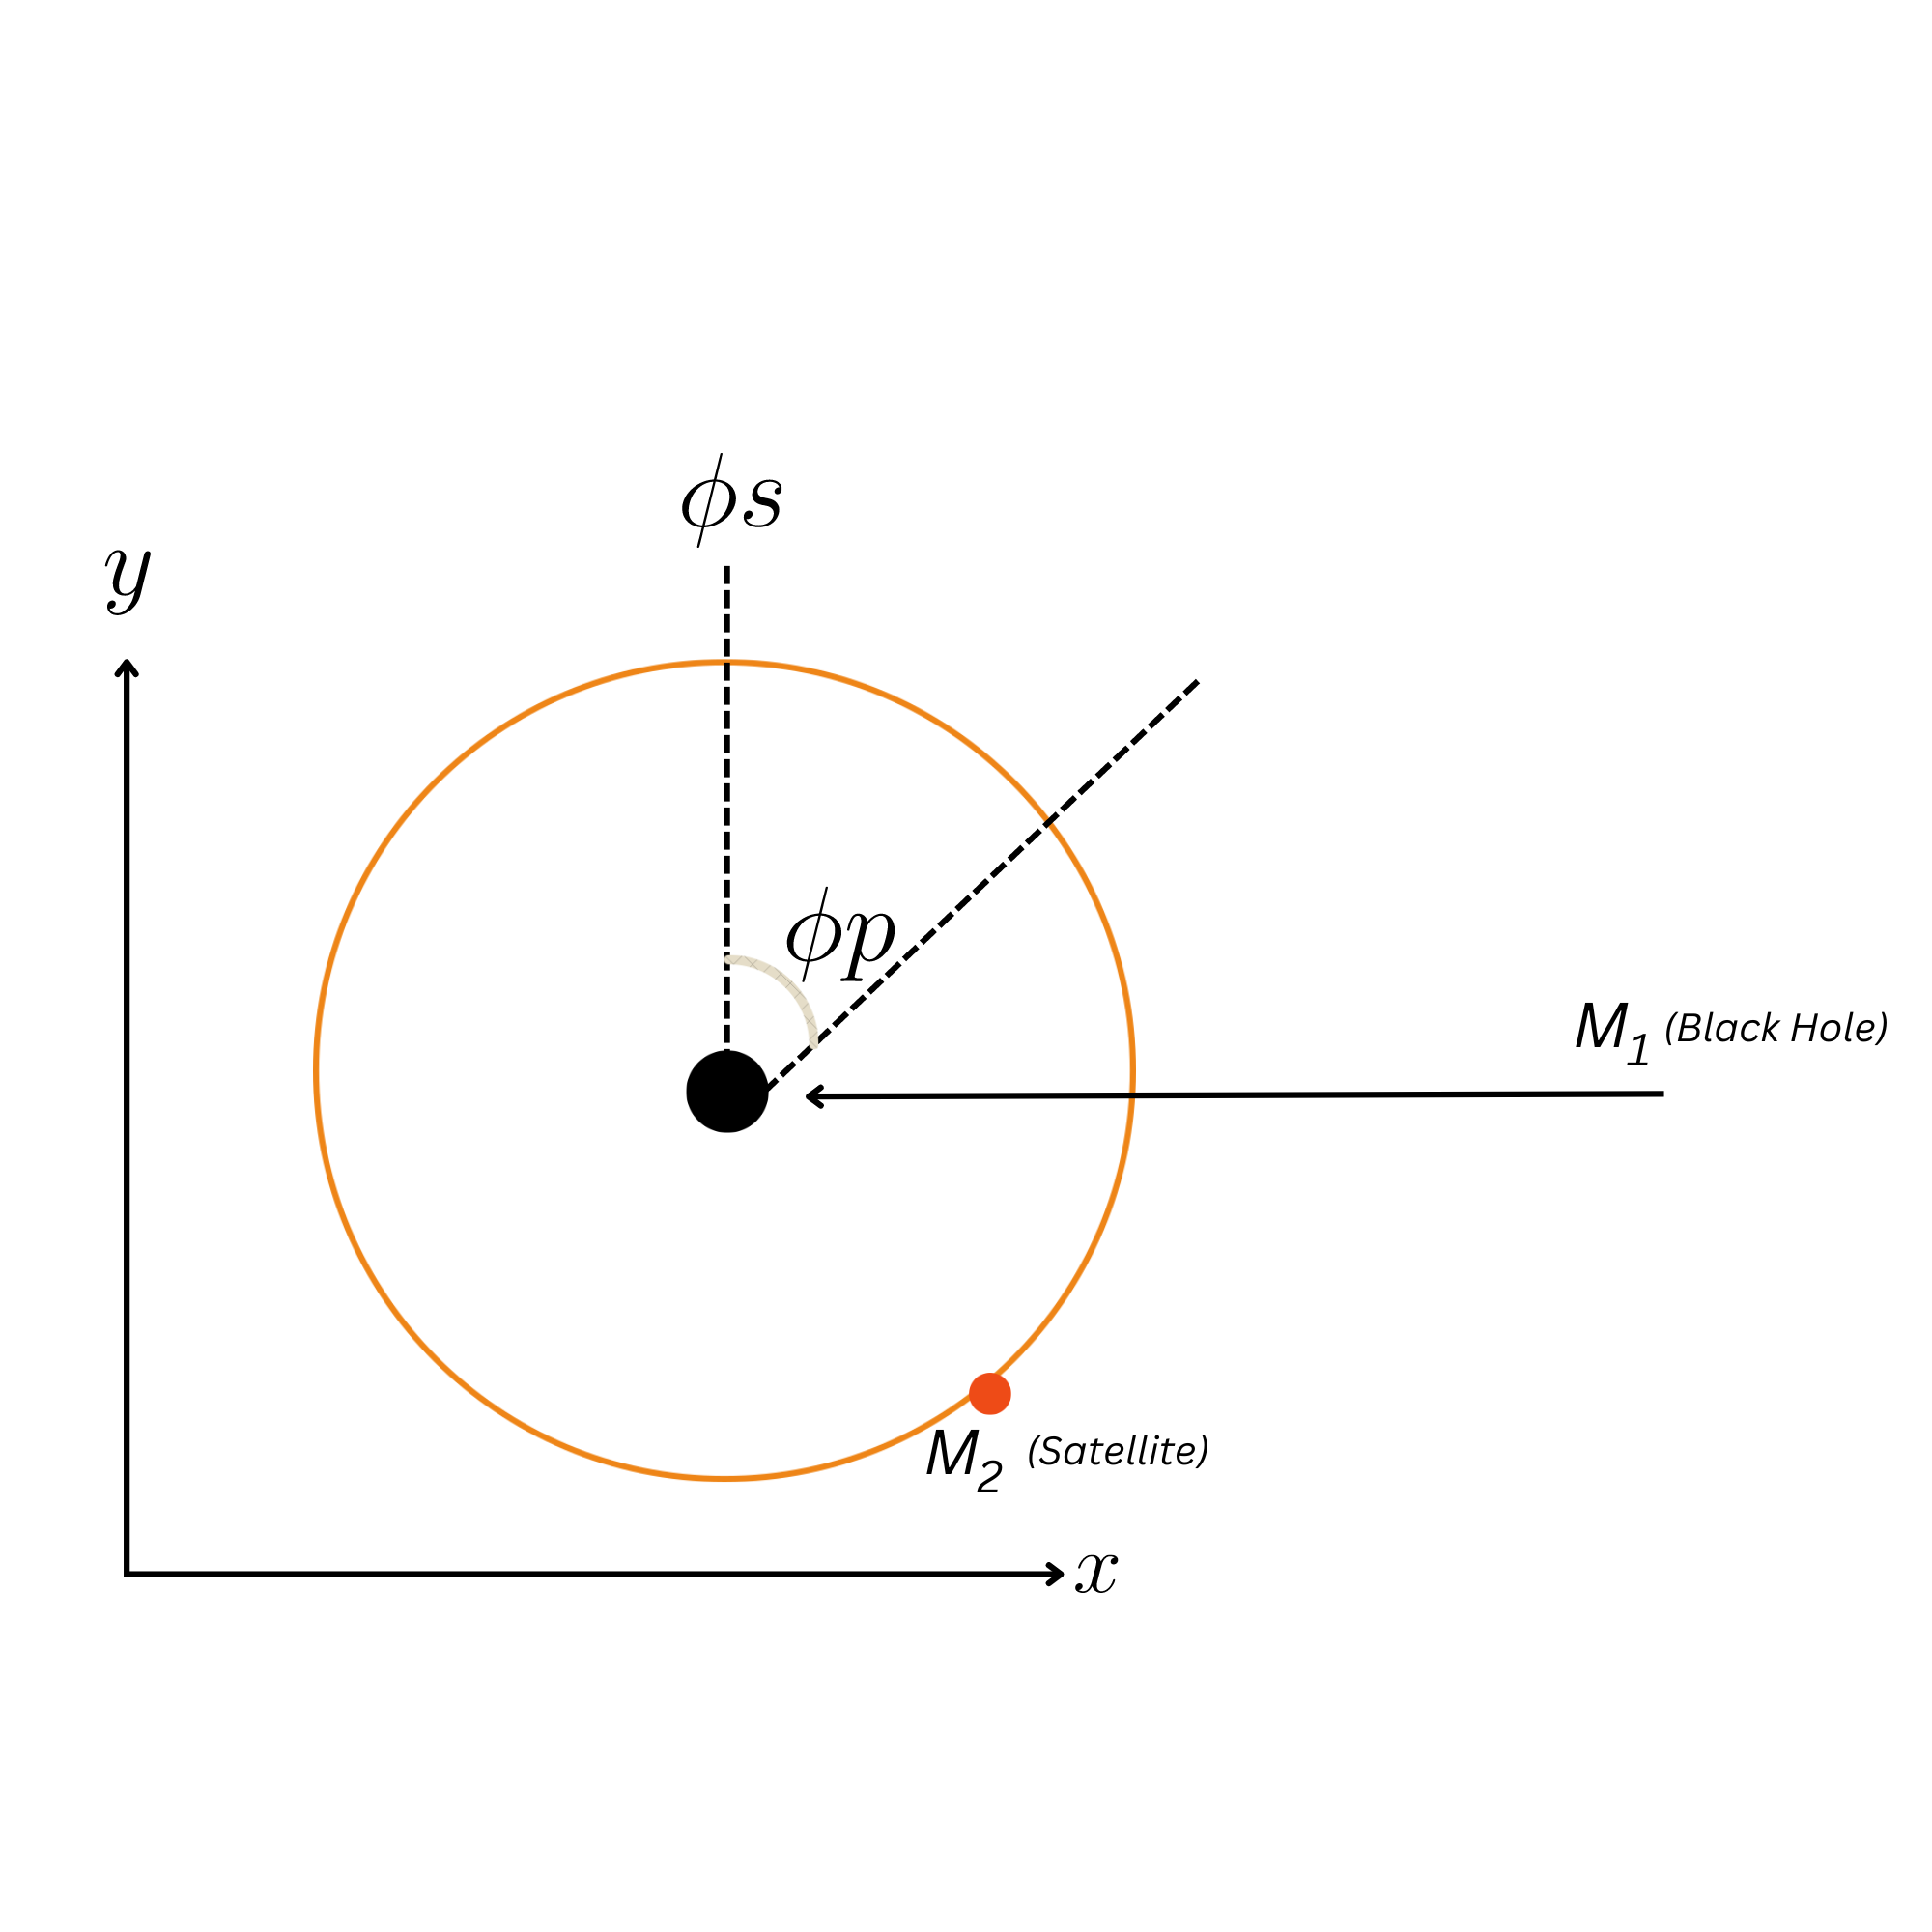
\includegraphics[width=10.5 cm]{Figures/SERPENS.png}
\caption{SERPENS utilizes a distinct geometrical and coordinate framework. Initially, the x-axis coincides with the alignment of the exoplanet and black hole at \( t = 0 \). As time proceeds, the exoplanet traverses its orbital path, governed by the true anomaly \( \phi_p \). The y-axis, situated within the orbital plane, stands orthogonal to the x-axis. Concurrently, the z-axis is aligned parallel to the orbital plane's specific angular momentum vector. The spatial position of the exomoon mirrors that of the exoplanet's coordinate system, albeit adjusted for the exoplanet's location. To effectively chart the exomoon's path, a reference frame that rotates in unison with the exoplanet is utilized.
\label{fig1}}
\end{figure}  
\subsubsection{Planetary Accretion}
We can approximate accretion as energy-limited Escape from an Exo-Io (Watson et al.\cite{Watson_1981}, demonstrated by atmospheric escape in the Kepler data (Jin et al. \cite{Jin_2014} and Fulton
\& Petigura\cite{Fulton_Petigura_2018}. This results in the hydrodynamic escape approximated by Oza et al. \cite{Oza_2019}
\begin{equation}
\dot{M}_U \sim m_i x_i \frac{Q}{U_s\left(R_a\right)} ,
\end{equation}
where,
\begin{equation}
Q=\eta_{\mathrm{XUV}} 4 \pi R_a^2 F_{\mathrm{XUV}} ,
\end{equation}
Note that we can use $\eta_{\mathrm{XUV}}$ = $0.1 - 0.4$ (eg., Murray-Clay et al. \cite{Murray-Clay_2009}). The escape flux may also be reduced if $Q_\mathrm{net}$ is too large as demonstrated by (Johnson et al. \cite{Johnson_2013_Erratum}):

\begin{equation}
Q_{\mathrm{net}}>Q_c \approx 4 \pi r_* \frac{\gamma}{c_c \sigma_c K n_m} \sqrt{\frac{2 U\left(r_*\right)}{m}} U\left(r_0\right) ,
\end{equation}

\subsubsection{Employing Particles}
For our analysis we employ a suite of particles formulated by Meyer zu Westram et al 2023 (submitted) \cite{Meyer_zu_Westram}. The velocity distribution follows a maxwell boltzman distribution with scaled parameter $v_{\mathrm{sc}}$ given by the distribution of $\chi^2$. 
\begin{equation}
    f_{\mathrm{th}}(v ; \mathbf{r})=\sqrt{\frac{2}{\pi}} \frac{v^2}{v_{\mathrm{sc}}^3} \exp \left(-\frac{v^2}{2 v_{\mathrm{sc}}^2}\right) ,
\end{equation}
where,
\begin{equation}
    v_{\mathrm{sc}}(\mathbf{r})=\sqrt{\frac{k_B T}{m}} ,
\end{equation}
The mass loss is determined by the ejection of particles $\mathrm{p}$. One such model was represented by Smyth and Combi \cite{osti_6642954} that combines the Boltzman distribution with a high-energy tail:  

\begin{equation}
f_{\mathrm{sp}}\left(v ; \alpha, v_b, v_M\right)=\frac{1}{D\left(\alpha, v_M / v_b\right)} \frac{1}{v_b} \cdot\left(\frac{v}{v_b}\right)^3\left(\frac{v_b^2}{v^2-v_b^2}\right)^\alpha \cdot\left(1-\sqrt{\frac{v^2+v_b^2}{v_M^2}}\right) ,
\end{equation}

where we have the dimensionless normalization constant

\begin{equation}
D\left(\alpha, v_M / v_b\right)=\int_0^{\sqrt{\left(v_M / v_b\right)^2-1}} \frac{x^3}{\left(1+x^2\right)^\alpha}\left(1-\frac{v_b}{v_M} \sqrt{1+x^2}\right) d x ,
\end{equation}

\subsubsection{Mass Loss}

SERPENS simulates reacions defined by their reaction rate at each advance, and the weight of a superparticle calculated as follows: 

\begin{equation}
   w(t)=e^{-t / \tau_1} e^{-t / \tau_2} \ldots e^{-t / \tau_n}, 
\end{equation}
with given lifetime $\tau_i=1 / \nu_i$ for the $i$-th reaction given the reaction rate $\nu_i$ \cite{Meyer_zu_Westram} 

These integrations are conducted through the REBOUND software (Rein and Liu \cite{Rein_Liu_2012}. Particles that are collided with an object due to gravitational interaction, would be therefore removed from analysis.

\subsubsection{Calculating Mixing Ratios}

The settling speed can be used to find the mixing ratio through the following relation from (Arras et al. \cite{Arras_2022}):

\begin{equation}
\frac{n}{n_{\mathrm{b}}} = \frac{F}{u n_{\mathrm{b}}} = -\frac{F \nu}{g n_{\mathrm{b}}} = -\frac{F\langle\sigma v\rangle}{g}
\end{equation}

where $F < 0$ for downward motion. Since the background density has canceled out of the right-hand side, the result will vary slowly with altitude.

The particle flux below the source can be written as:

\begin{equation}
\begin{aligned}
F & =-f_{\mathrm{pl}} \epsilon_{\mathrm{abl}} f \frac{\dot{M}{\mathrm{d}}}{4 \pi R{\mathrm{p}}^2 \bar{m}} \
& \simeq-6.5 \times 10^9 \mathrm{~cm}^{-2} \mathrm{~s}^{-1} f\left(\frac{f_{\mathrm{pl}} \epsilon_{\mathrm{abl}} \dot{M}{\mathrm{d}}}{10^8 \mathrm{~g} \mathrm{~s}^{-1}}\right)\left(\frac{R{\mathrm{p}}}{R_{\mathrm{J}}}\right)^{-2} .
\end{aligned}
\end{equation}

Here, $\dot{M_d}$ is the accretion rate of the dust population as it moves toward the star under PR drag, $f$ is the abundance by number of this element in the dust particles, and $\bar{m}$ is the mean mass of the elements making up the dust particles.

The results are now assembled to compute the mixing ratio below the meteoric source. The result is:

\begin{equation}
\begin{aligned}
\frac{n}{n_{\mathrm{b}}} = & 4.1 \times 10^{-3} f\left(\frac{f_{\mathrm{pl}} \epsilon_{\mathrm{abl}} \dot{M}{\mathrm{d}}}{10^8 \mathrm{~g} \mathrm{~s}^{-1}}\right) \
& \times\left(\frac{M{\mathrm{p}}}{M_{\mathrm{J}}}\right)^{-1}\left(\frac{T}{10^3 \mathrm{~K}}\right)^{1 / 2}\left(\frac{m_{\mathrm{b}} m_{\mathrm{u}}}{m\left(m+m_{\mathrm{b}}\right)}\right)^{1 / 2} .
\end{aligned}
\end{equation}

The relative number of different elements scales as $f/m$ for $m > m_b$, and favor small planets due to the smaller gravity.

\begin{figure}[H]
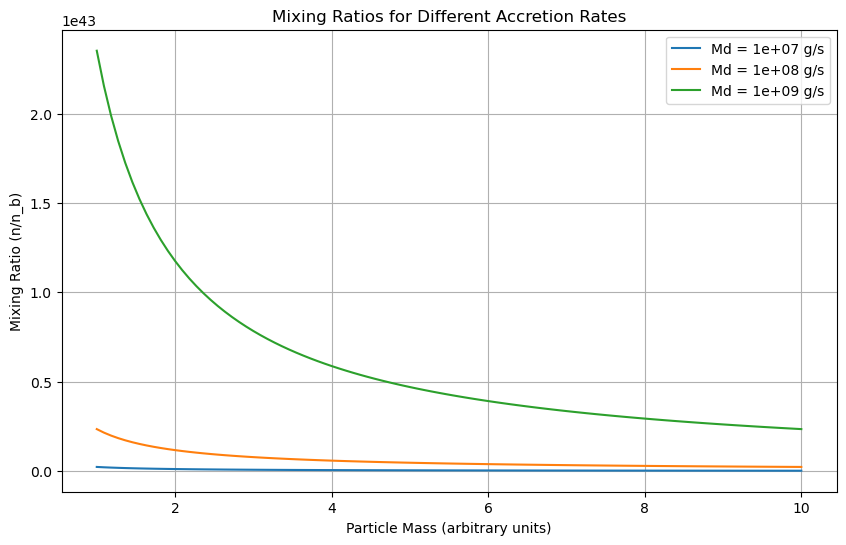
\includegraphics[width=10.5 cm]{Figures/mixing_ratios.png}
\caption{Mixing Ratio Analytical Approximation at $\dot{M}$ $=$ $10^7$, $10^8$, and $10^9$ to validate model.
\label{fig2}}
\end{figure}  

%%%%%%%%%%%%%%%%
\subsubsection{Estimating the number density of the background gas}
%%%%%%%%%%%%%%%%
\textbf{The background gas n$_b$ can be written as if the gas is ideal:}

\begin{equation}
    n_b \sim P_{b,atm}/k_b/T_{b,atm}
\end{equation}

Where we assume that T$_{b,atm} \sim$ T$_{eq}$ of the exoplanet atmosphere, and the maximum gas pressure probed in transmission is roughly P$_{b,atm} \sim$ 1 mbar.


\subsection{Accretion Rate in a Black Hole}

For a Black Hole system, we must adjust our accretion rate accordingly. The central object accrediting at some rate $\Mdot$, given by an accretion power:

\begin{equation}
    L_{\mathrm{acc}}=\frac{G M \dot{M}}{R}
\end{equation}

The Eddington accretion rate is the maximum rate at which a black hole can accrete matter without the inward gravitational pull being overcome by the outward force due to radiation pressure from the accreting matter \cite{Armitage_2004}. This radiation pressure is a consequence of photon scattering off free electrons in the accretion flow. The Eddington luminosity is defined as the luminosity at which the radiation pressure balances the gravitational force exerted on the accreting matter.

The Eddington luminosity ($L_{\text{Edd}}$) is given by the equation:

\begin{equation}
L_{\text{Edd}} = \frac{4 \pi G M c}{\sigma_T}
\end{equation}

In this context, $G$ is the gravitational constant, $M$ is the mass of the black hole, $c$ is the speed of light, and $\sigma_T$ is the Thomson scattering cross-section. The Eddington luminosity represents the point at which the radiation pressure from the black hole equals the gravitational pull of the black hole on a unit of gas at its surface.

Following from this, the Eddington accretion rate ($\dot{M}_{\text{Edd}}$) can then be expressed as:

\begin{equation}
\dot{M}{_\text{Edd}} = \frac{L{_\text{Edd}}}{\varepsilon c^2}
\end{equation}

In this equation, $\varepsilon$ is the radiative efficiency, which is a measure of the fraction of the accreted mass that is converted into radiation. The value of $\varepsilon$ can vary depending on the specific properties of the black hole. The Black Hole system SS433 provides evidence for for these outflows, discovered by (Stephenson \& Sanduleak \cite{Stephenson_Sanduleak_1977}). For a non-spinning, or Schwarzschild, black hole, $\varepsilon$ is typically around 0.1 (Frank et al. \cite{Frank_King_Raine_2002}, signifying that about 10 percent of the accreted mass is converted into radiation.

Therefore the Eddington Accretion Rate is: 
\begin{equation}
    \dot{M}_{\mathrm{Edd}}=\frac{4 \pi G M_{\mathrm{BH}} m_{\mathrm{p}}}{\varepsilon \sigma_{\mathrm{T}} c}
\end{equation}

Where $M_{\mathrm{BH}}$ is the Mass of the Black Hole.



%%%%%%%%%%%%%%%%%%%%%%%%%%%%%%%%%%%%%%%%%%
\section{Results}



%%%%%%%%%%%%%%%%%%%%%%%%%%%%%%%%%%%%%%%%%%
\section{Discussion}

Authors should discuss the results and how they can be interpreted from the perspective of previous studies and of the working hypotheses. The findings and their implications should be discussed in the broadest context possible. Future research directions may also be highlighted.

%%%%%%%%%%%%%%%%%%%%%%%%%%%%%%%%%%%%%%%%%%
\section{Conclusions}

This section is not mandatory, but can be added to the manuscript if the discussion is unusually long or complex.

%%%%%%%%%%%%%%%%%%%%%%%%%%%%%%%%%%%%%%%%%%


%%%%%%%%%%%%%%%%%%%%%%%%%%%%%%%%%%%%%%%%%%
\vspace{6pt} 

%%%%%%%%%%%%%%%%%%%%%%%%%%%%%%%%%%%%%%%%%%
%% optional
%\supplementary{The following supporting information can be downloaded at:  \linksupplementary{s1}, Figure S1: title; Table S1: title; Video S1: title.}

% Only for journal Methods and Protocols:
% If you wish to submit a video article, please do so with any other supplementary material.
% \supplementary{The following supporting information can be downloaded at: \linksupplementary{s1}, Figure S1: title; Table S1: title; Video S1: title. A supporting video article is available at doi: link.}

% Only for journal Hardware:
% If you wish to submit a video article, please do so with any other supplementary material.
% \supplementary{The following supporting information can be downloaded at: \linksupplementary{s1}, Figure S1: title; Table S1: title; Video S1: title.\vspace{6pt}\\
%\begin{tabularx}{\textwidth}{lll}
%\toprule
%\textbf{Name} & \textbf{Type} & \textbf{Description} \\
%\midrule
%S1 & Python script (.py) & Script of python source code used in XX \\
%S2 & Text (.txt) & Script of modelling code used to make Figure X \\
%S3 & Text (.txt) & Raw data from experiment X \\
%S4 & Video (.mp4) & Video demonstrating the hardware in use \\
%... & ... & ... \\
%\bottomrule
%\end{tabularx}
%}

%%%%%%%%%%%%%%%%%%%%%%%%%%%%%%%%%%%%%%%%%%
\authorcontributions{For research articles with several authors, a short paragraph specifying their individual contributions must be provided. The following statements should be used ``Conceptualization, X.X. and Y.Y.; methodology, X.X.; software, X.X.; validation, X.X., Y.Y. and Z.Z.; formal analysis, X.X.; investigation, X.X.; resources, X.X.; data curation, X.X.; writing---original draft preparation, X.X.; writing---review and editing, X.X.; visualization, X.X.; supervision, X.X.; project administration, X.X.; funding acquisition, Y.Y. All authors have read and agreed to the published version of the manuscript.'', please turn to the  \href{http://img.mdpi.org/data/contributor-role-instruction.pdf}{CRediT taxonomy} for the term explanation. Authorship must be limited to those who have contributed substantially to the work~reported.}



% Only for journal Nursing Reports
%\publicinvolvement{Please describe how the public (patients, consumers, carers) were involved in the research. Consider reporting against the GRIPP2 (Guidance for Reporting Involvement of Patients and the Public) checklist. If the public were not involved in any aspect of the research add: ``No public involvement in any aspect of this research''.}

% Only for journal Nursing Reports
%\guidelinesstandards{Please add a statement indicating which reporting guideline was used when drafting the report. For example, ``This manuscript was drafted against the XXX (the full name of reporting guidelines and citation) for XXX (type of research) research''. A complete list of reporting guidelines can be accessed via the equator network: \url{https://www.equator-network.org/}.}

\acknowledgments{In this section you can acknowledge any support given which is not covered by the author contribution or funding sections. This may include administrative and technical support, or donations in kind (e.g., materials used for experiments).}

\conflictsofinterest{The authors declare no conflicts of interest.} 

%%%%%%%%%%%%%%%%%%%%%%%%%%%%%%%%%%%%%%%%%%
%% Optional

%% Only for journal Encyclopedia
%\entrylink{The Link to this entry published on the encyclopedia platform.}




%%%%%%%%%%%%%%%%%%%%%%%%%%%%%%%%%%%%%%%%%%
\begin{adjustwidth}{-\extralength}{0cm}
%\printendnotes[custom] % Un-comment to print a list of endnotes

\reftitle{References}

% Please provide either the correct journal abbreviation (e.g. according to the “List of Title Word Abbreviations” http://www.issn.org/services/online-services/access-to-the-ltwa/) or the full name of the journal.
% Citations and References in Supplementary files are permitted provided that they also appear in the reference list here. 

%=====================================
% References, variant A: external bibliography
%=====================================
%\bibliography{your_external_BibTeX_file}

%=====================================
% References, variant B: internal bibliography
%=====================================
\begin{thebibliography}{999}
% Reference 1
\bibitem[Doyle et al.(2021)]{Doyle_2021}
Doyle, A.E.; Desch, S.J.; Young, E.D. Icy Exomoons Evidenced by Spallogenic Nuclides in Polluted White Dwarfs. {\em The Astrophysical Journal} {\bf 2021}, {\em 907}, L35.
\bibitem[Oza et al.(2019)]{Oza_2019}
Oza, A.V.; Johnson, R.E.; Lellouch, E.; Schmidt, C.; Schneider, N.; Huang, C.; Gamborino, D.; Gebek, A.; Wyttenbach, A.; Demory, B.-O. Sodium and Potassium Signatures of Volcanic Satellites Orbiting Close-in Gas Giant Exoplanets. {\em The Astrophysical Journal} {\bf 2019}, {\em 885}, 168.
\bibitem[Meyer zu Westram et al. (2023)]{Meyer_zu_Westram}
Meyer zu Westram, M.; Oza, A.V.; Galli, A. Exomoon Phase Curves: Toroidal Exosphere Simulations of Exo-Ios Orbiting Exoplanets in Alkali Spectroscopy. Manuscript submitted to {\em JGR: Planets}.
\bibitem[Watson et al.(1981)]{Watson_1981}
Watson, A.J.; Donahue, T.M.; Walker, J.C.G. 1981. {\em Icarus} {\bf 1981}, {\em 48}, 150.
\bibitem[Jin et al.(2014)]{Jin_2014}
Jin, S.; Mordasini, C.; Parmentier, V.; van Boekel, R.; Henning, T.; Ji, J. Planetary Population Synthesis Coupled with Atmospheric Escape: A Statistical View of Evaporation. {\em The Astrophysical Journal} {\bf 2014}, {\em 795}, 65.
\bibitem[Fulton and Petigura(2018)]{Fulton_Petigura_2018}
Fulton, B.J.; Petigura, E.A. The California-Kepler Survey. VII. Precise Planet Radii Leveraging Gaia DR2 Reveal the Stellar Mass Dependence of the Planet Radius Gap. {\em The Astronomical Journal} {\bf 2018}, {\em 156}, 264.
\bibitem[Murray-Clay et al.(2009)]{Murray-Clay_2009}
Murray-Clay, R.A.; Chiang, E.I.; Murray, N. Atmospheric Escape From Hot Jupiters. {\em The Astrophysical Journal} {\bf 2009}, {\em 693}, 23-42.
\bibitem[Johnson et al.(2013)]{Johnson_2013_Erratum}
Johnson, R.E.; Volkov, A.N.; Erwin, J.T. Erratum: “Molecular–Kinetic Simulations of Escape from the Ex-Planet and Exoplanets: Criterion for Transonic Flow” (2013, ApJL, 768, L4). {\em The Astrophysical Journal Letters} {\bf 2013}, {\em 779}, L30.
\bibitem[Armitage(2004)]{Armitage_2004}
Armitage, P.J. Theory of Disk Accretion onto Supermassive Black Holes. In {\em Supermassive Black Holes in the Distant Universe}; Springer Netherlands: 2004; pp. 89--126.
\bibitem[Rees(1988)]{Rees_1988}
Rees, M.J. Tidal disruption of stars by black holes of 10 to the 6th-10 to the 8th solar masses in nearby galaxies. {\em Nature} {\bf 1988}, {\em 333}, 523--528.
\bibitem[Pringle(1981)]{Pringle_1981}
Pringle, J.E. Accretion Discs in Astrophysics. {\em Annual Review of Astronomy and Astrophysics} {\bf 1981}, {\em 19}, 137--160.
\bibitem[Arras et al.(2022)]{Arras_2022}
Arras, P.; Wilson, M.; Pryal, M.; Baker, J. Dust Accretion onto Exoplanets. {\em The Astrophysical Journal} {\bf 2022}, {\em 932}, 90.
\bibitem[Blandford and Payne(1982)]{Blandford_Payne_1982}
Blandford, R.D.; Payne, D.G. Hydromagnetic flows from accretion disks and the production of radio jets. {\em Monthly Notices of the Royal Astronomical Society} {\bf 1982}, {\em 199}, 883-903.
\bibitem[Smyth and Combi(1988)]{osti_6642954}
Smyth, W.H.; Combi, M.R. Extended atmospheres of outer planet satellites and comets. Final report, 1 August 1984-31 August 1988. 1988.
\bibitem[Rein and Liu(2012)]{Rein_Liu_2012}
Rein, H.; Liu, S.-F. REBOUND: An Open-Source Multi-purpose N-body Code for Collisional Dynamics. {\em Astronomy & Astrophysics} {\bf 2012}, {\em 537}, A128.
\bibitem[Frank et al.(2002)]{Frank_King_Raine_2002}
Frank, J.; King, A.; Raine, D. Accretion Power in Astrophysics. 3rd ed.; Cambridge University Press: Cambridge, 2002; doi:10.1017/CBO9781139164245.
\bibitem[Stephenson and Sanduleak(1977)]{Stephenson_Sanduleak_1977}
Stephenson, C.B.; Sanduleak, N. New H-alpha Emission Stars in the Milky Way. {\em Astrophysical Journal, Supplement Series} {\bf 1977}, {\em 33}, 459-469.
\end{thebibliography}

% If authors have biography, please use the format below
%\section*{Short Biography of Authors}
%\bio
%{\raisebox{-0.35cm}{\includegraphics[width=3.5cm,height=5.3cm,clip,keepaspectratio]{Definitions/author1.pdf}}}
%{\textbf{Firstname Lastname} Biography of first author}
%
%\bio
%{\raisebox{-0.35cm}{\includegraphics[width=3.5cm,height=5.3cm,clip,keepaspectratio]{Definitions/author2.jpg}}}
%{\textbf{Firstname Lastname} Biography of second author}

% For the MDPI journals use author-date citation, please follow the formatting guidelines on http://www.mdpi.com/authors/references
% To cite two works by the same author: \citeauthor{ref-journal-1a} (\citeyear{ref-journal-1a}, \citeyear{ref-journal-1b}). This produces: Whittaker (1967, 1975)
% To cite two works by the same author with specific pages: \citeauthor{ref-journal-3a} (\citeyear{ref-journal-3a}, p. 328; \citeyear{ref-journal-3b}, p.475). This produces: Wong (1999, p. 328; 2000, p. 475)

%%%%%%%%%%%%%%%%%%%%%%%%%%%%%%%%%%%%%%%%%%
%% for journal Sci
%\reviewreports{\\
%Reviewer 1 comments and authors’ response\\
%Reviewer 2 comments and authors’ response\\
%Reviewer 3 comments and authors’ response
%}
%%%%%%%%%%%%%%%%%%%%%%%%%%%%%%%%%%%%%%%%%%
\PublishersNote{}
\end{adjustwidth}
\end{document}

